\documentclass[handout]{beamer}

\usepackage[utf8]{inputenc}
\usepackage[english,russian]{babel}
\usepackage{listings}

%\ifx\pdftexversion\undefined
%\usepackage[dvips]{graphicx}
%\else
%\usepackage[pdftex]{graphicx}
%\DeclareGraphicsRule{*}{mps}{*}{}
%#\fi

\definecolor{javared}{rgb}{0.6,0,0} % for strings
\definecolor{javagreen}{rgb}{0.25,0.5,0.35} % comments
\definecolor{javapurple}{rgb}{0.5,0,0.35} % keywords
\definecolor{javadocblue}{rgb}{0.25,0.35,0.75} % javadoc
 
\lstset{language=Java,
basicstyle=\footnotesize\ttfamily,
keywordstyle=\color{javapurple}\bfseries,
stringstyle=\color{javared},
commentstyle=\color{javagreen},
morecomment=[s][\color{javadocblue}]{/**}{*/},
stepnumber=2,
numbersep=10pt,
tabsize=4,
showspaces=false,
showstringspaces=false}


\title{Паттерны Iterator, Command}
\author{Есилевич Александр}

\begin{document}

\maketitle

\begin{frame}[fragile]
\frametitle{Векторный графический редактор}
\begin{itemize}
\item Манипулирование графическими примитивами, а не точками (пикселями)
\item Интерактивность — добавление и редактирование графических примитивов мышью
\item Легкость расширения и портирования на разные платформы
\end{itemize}
\end{frame}


\begin{frame}[fragile]
\frametitle{Средства, предоставляемые графической библиотекой}
\begin{itemize}
\item \lstinline{class SystemComponent} — базовый элемент графического интерфейса
\item \lstinline{class SystemWindow} — окно приложения
\item \lstinline{class SystemCanvas} — «холст», объект для отображения содержимого компонентов
\item Набор примитивных графических элементов управления (надписи, кнопки, текстовые поля, списки)
\end{itemize}
\end{frame}


\begin{frame}[fragile]
\frametitle{Структура графического интерфейса}
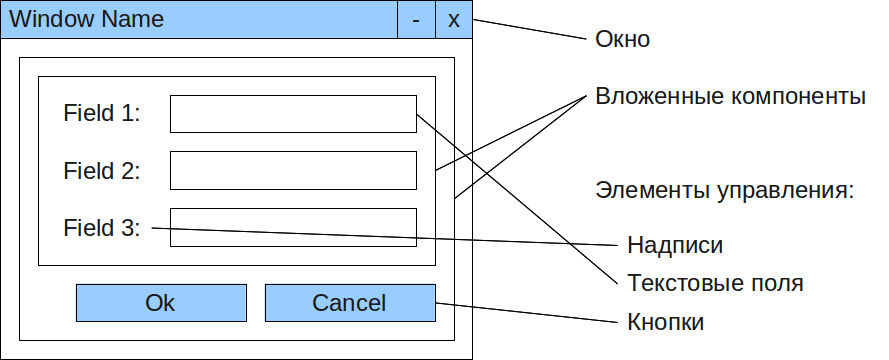
\includegraphics[scale=0.5]{window.png}
\end{frame}


\begin{frame}[fragile]
\frametitle{Класс SystemComponent}
\begin{lstlisting}
public abstract class SystemComponent {

    public abstract void paint(SystemCanvas canvas);

    public void handleMousePress(int x, int y) {}
    public void handleMouseRelease(int x, int y) {}
    public void handleMouseMove(int x, int y) {}
    public void handleMouseClick(int x, int y) {}
    public void handleKeyPress(char c) {}

    // Other mouse/keyboard events
    // ...
}
\end{lstlisting}
\end{frame}


\begin{frame}[fragile]
\frametitle{Класс SystemCanvas}
\begin{lstlisting}
public class SystemCanvas {

    public void drawLine(int x1, int y1,
                         int x2, int y2);

    public void drawOval(int x, int y,
                         int width, int height);

    // Other graphics primitives
}
\end{lstlisting}
\end{frame}


\begin{frame}[fragile]
\frametitle{Java AWT - Abstract Window Toolkit}
\begin{itemize}
\item \lstinline{SystemWindow} = \lstinline{java.awt.Frame}
\item \lstinline{SystemComponent} = \lstinline{java.awt.Component}
\item \lstinline{SystemCanvas} = \lstinline{java.awt.Graphics}
\end{itemize}
\end{frame}


\begin{frame}[fragile]
\begin{center}
\huge С чего начать?
\end{center}
\end{frame}


\begin{frame}[fragile]
\frametitle{Диаграмма классов геометрических фигур}
\begin{center}
\includegraphics{shape.mps}
\end{center}
\end{frame}


\begin{frame}[fragile]
\frametitle{Класс для представления фигуры}
\begin{lstlisting}
public abstract class Shape {
    public abstract void draw(SystemCanvas canvas);
}
\end{lstlisting}
\end{frame}


\begin{frame}[fragile]
\frametitle{Линия}
\begin{lstlisting}
public class Line extends Shape {

    public Line(int px1, int py1, int px2, int py2) {
        x1 = px1;
        y1 = py1;
        x2 = px2;
        y2 = py2;
    }

    public void draw(SystemCanvas canvas) {
        canvas.drawLine(x1, y1, x2, y2);
    }

    private int x1;
    private int y1;
    private int x2;
    private int y2;
}
\end{lstlisting}
\end{frame}


\begin{frame}[fragile]
\frametitle{Прямоугольник}
\begin{lstlisting}
public class Rectangle extends Shape {
    public Rectangle(int px1, int py1,
                     int px2, int py2) {
        x1 = px1;
        y1 = py1;
        x2 = px2;
        y2 = py2;
    }

    public void draw(SystemCanvas canvas) {
        canvas.drawLine(x1, y1, x2, y1);
        canvas.drawLine(x2, y1, x2, y2);
        canvas.drawLine(x2, y2, x1, y2);
        canvas.drawLine(x1, y2, x1, y1);
    }

    private int x1;
    private int y1;
    private int x2;
    private int y2;
}
\end{lstlisting}
\end{frame}


\begin{frame}[fragile]
\frametitle{Окружность}
\begin{lstlisting}
public class Circle extends Shape {

    public Circle(int px, int py, int pradius) {
        x = px;
        y = py;
        radius = pradius;
    }

    public void draw(SystemCanvas canvas) {
        canvas.drawOval(x - radius, y - radius,
                        x + radius, y + radius);
    }

    private int x;
    private int y;
    private int radius;
}
\end{lstlisting}
\end{frame}


\begin{frame}[fragile]
\frametitle{Пример использования класса Shape}
\begin{lstlisting}
public class MyComponent extends SystemComponent {

    public void paint(SystemCanvas canvas) {
        Shape line = new Line(10, 10, 20, 20);
        line.draw(canvas);

        Shape circle = new Circle(100, 100, 40);
        circle.draw(canvas);

        Rectangle rect = new Rectangle(30, 30, 50, 50)
        rect.draw(canvas);
    }
}
\end{lstlisting}
\end{frame}


\begin{frame}[fragile]
\begin{center}
\huge Как хранить коллекцию фигур?
\end{center}
\end{frame}


\begin{frame}[fragile]
\frametitle{Двусвязный список}
\begin{center}
\includegraphics{shape_list.mps}
\end{center}
\end{frame}


\begin{frame}[fragile]
\frametitle{Класс Scene}
\begin{lstlisting}
public class Scene extends SystemComponent {
    public void paint(SystemCanvas canvas) {
        Shape shape = first;
        while(shape != null) {
            shape.draw(graphics);
            shape = shape.next;
        }
    }

    public void addShape(Shape shape);
    public void addShapeBefore(Shape s, Shape before);
    public void removeShape(Shape s);

    private Shape first;
    private Shape last;
}
\end{lstlisting}
\end{frame}


\begin{frame}[fragile]
\frametitle{Класс Scene}
\begin{lstlisting}
public void addShape(Shape shape) {
    if(first == null) {
        // no items in the list
        first = shape;
        last = shape;
    } else {
        last.next = shape;
        shape.prev = last;
        last = shape;
    }
}
\end{lstlisting}
\end{frame}


\begin{frame}[fragile]
\frametitle{Класс Scene}
\begin{lstlisting}
public void addShapeBefore(Shape s, Shape before) {

    Shape shape = first;
    while(shape != null) {
        if(shape == before) {
            s.next = shape;

            if(shape.prev != null) {
                shape.prev.next = s;
                s.prev = shape.prev;
            } else {
                first = s;
            }

            shape.prev = s;
            break;
        }

        shape = shape.next;
    }
}
\end{lstlisting}
\end{frame}


\begin{frame}[fragile]
\frametitle{Класс Scene}
\begin{lstlisting}
    public void removeShape(Shape s) {
        Shape shape = first;
        while(shape != null) {
            if(shape == s) {
                if(shape == first && shape == last) {
                    first = null;
                    last = null;
                } else if(shape == first) {
                    first = shape.next;
                    shape.next.prev = null;
                } else if(shape == last) {
                    last = shape.prev;
                    shape.prev.next = null;
                } else {
                    shape.prev.next = shape.next;
                    shape.next.prev = shape.prev;
                }
            }
            shape = shape.next;
        }
    }
\end{lstlisting}
\end{frame}


\begin{frame}[fragile]
\frametitle{Недостатки}
\begin{itemize}
\item Класс \lstinline{Shape} предполагает наличие двусвязного списка,
      т. к. имеет поля \lstinline{prev} и \lstinline{next}
\item Открытые (\lstinline{public}) поля \lstinline{prev}, \lstinline{next}
\item Нельзя переиспользовать операции работы со списком фигур,
      т. к. они привязаны к классу \lstinline{Scene}
\item Класс \lstinline{Scene} зависит от внутренней структуры списка
\end{itemize}
\end{frame}


\begin{frame}[fragile]
\frametitle{Двусвязный список + ShapeListItem}
\begin{center}
\includegraphics{shape_list_item.mps}
\end{center}
\end{frame}


\begin{frame}[fragile]
\frametitle{Класс ShapeListItem}
\begin{lstlisting}
public class ShapeListItem {

    public ShapeListItem(Shape s);
    public Shape getShape();
    public void setShape(Shape s);

    ShapeListItem getNext();
    void setNext(ShapeListItem item);

    ShapeListItem getPrev();
    void setPrev(ShapeListItem item);

    private Shape shape;
    private ShapeListItem prev;
    private ShapeListItem next;
}
\end{lstlisting}
\end{frame}


\begin{frame}[fragile]
\frametitle{Класс Scene - модификация 1}
\begin{lstlisting}
public void addShape(Shape shape) {
    ShapeListItem item = new ShapeListItem(shape);
    // add item to the list
}
\end{lstlisting}
\end{frame}


\begin{frame}[fragile]
\frametitle{Класс Scene - модификация 1}
\begin{lstlisting}
public void addShapeBefore(Shape s, Shape before) {
    ShapeListItem newItem = new ShapeListItem(s);
    ShapeListItem item = first;
    while(item != null) {
        if(item.getShape() == before) {
            // add item to the list
        }
        item = item.getNext();
    }
}
\end{lstlisting}
\end{frame}


\begin{frame}[fragile]
\frametitle{Класс Scene - модификация 1}
\begin{lstlisting}
public void removeShape(Shape s) {
    ShapeListItem item = first;
    while(item != null) {
        if(item.getShape() == s) {
            // remove item from the list
        }
        item = item.getNext();
    }
}
\end{lstlisting}
\end{frame}


\begin{frame}[fragile]
\frametitle{Класс ShapeList}
\begin{lstlisting}
public class ShapeList {
    public void add(Shape shape);
    public void addBefore(Shape s, ShapeListItem before);
    public void remove(ShapeListItem item);

    public ShapeListItem getFirst();

    private ShapeListItem first;
    private ShapeListItem last;
}
\end{lstlisting}
\end{frame}


\begin{frame}[fragile]
\frametitle{Класс Scene - модификация 2}
\begin{lstlisting}
public void addShape(Shape shape) {
    shapes.add(shape);
}
\end{lstlisting}
\end{frame}


\begin{frame}[fragile]
\frametitle{Класс Scene - модификация 2}
\begin{lstlisting}
public void addShapeBefore(Shape s, Shape before) {
    ShapeListItem item = shapes.getFirst();
    while(item != null) {
        if(item.getShape() == before) {
            shapes.addBefore(s, item);
            break;
        }

        item = item.getNext();
    }
}
\end{lstlisting}
\end{frame}


\begin{frame}[fragile]
\frametitle{Класс Scene - модификация 2}
\begin{lstlisting}
public void removeShape(Shape s) {
    ShapeListItem item = shapes.getFirst();
    while(item != null) {
        if(item.getShape() == before) {
            shapes.addBefore(s, item);
            break;
        }

        item = item.getNext();
    }
}
\end{lstlisting}
\end{frame}


\begin{frame}[fragile]
\frametitle{Диаграмма классов}
\begin{center}
\includegraphics{class_diag.mps}
\end{center}
\end{frame}


\begin{frame}[fragile]
\frametitle{Внешний интерфейс класса ShapeListItem}
\begin{lstlisting}
public class ShapeListItem {
    public Shape getShape();
    public void setShape(Shape s);

    ShapeListItem getNext();
}
\end{lstlisting}
\end{frame}


\begin{frame}[fragile]
\frametitle{Класс ShapeListItem + ShapeListNode}
\begin{lstlisting}
public class ShapeListItem {
    public ShapeListItem(PrivateShapeListItem i) {
        item = i;
    }
    public Shape getShape() {
        return item.getShape();
    }
    public ShapeListItem getNext() {
        if(item.getNext() == null)
            return null;

        return new ShapeListItem(item.getNext());
    }
    // for internal use only
    public PrivateShapeListItem getPrivateItem() {
        return item;
    }
    private ShapeListNode node;
}
\end{lstlisting}
\end{frame}


\begin{frame}[fragile]
\frametitle{Диаграмма классов с ShapeListNode}
\begin{center}
\includegraphics{class_diag2.mps}
\end{center}
\end{frame}


\begin{frame}[fragile]
\frametitle{Паттерн Iterator}
\begin{center}
\includegraphics{class_diag_iterator.mps}
\end{center}
\end{frame}


\begin{frame}[fragile]
\frametitle{Массив вместо списка}
\begin{lstlisting}
public class ShapeListIterator {
    public Shape getShape() {
        assert(!isEnd());
        return array[index];
    }
    public ShapeListIterator getNext() {
        assert(!isEnd());
        return new ShapeListIterator(array, index + 1);
    }
    public boolean isEnd() {
        return index >= array.length;
    }

    Shape [] array;
    private int index;
}
\end{lstlisting}
\end{frame}


\begin{frame}[fragile]
\frametitle{Массив вместо списка}
\begin{lstlisting}
public class ShapeList {

    public ShapeListIterator getFirst() {
        return new ShapeListIterator(array, 0);
    }

    private Shape [] array;
};
\end{lstlisting}
\end{frame}


\begin{frame}[fragile]
\frametitle{Виды итераторов}
\begin{itemize}
\item Создаётся контейнером или клиентом?
\item Для доступа к элементу нужно вызвать метод итератора или контейнера?
\item Может ли итератор изменять элементы?
\item Для изменения элемента нужно вызвать метод итератора или контейнера?
\item Отделена ли итерация от доступа к элементу?
\end{itemize}
\end{frame}


\begin{frame}[fragile]
\frametitle{C++ Iterator}
\begin{lstlisting}
public class ShapeIterator {
    public ShapeListIterator getNext();
    public Shape getShape();
};
\end{lstlisting}
\end{frame}


\begin{frame}[fragile]
\frametitle{Java Iterator}
\begin{lstlisting}
public class ShapeIterator {
    public Shape getNext();
    public bool isEnd();
};
\end{lstlisting}
\end{frame}



\begin{frame}[fragile]
\frametitle{Абстрактный итератор}
\begin{center}
\includegraphics{class_diag_aiterator.mps}
\end{center}
\end{frame}


\begin{frame}[fragile]
\frametitle{Результаты}
\begin{itemize}
\item Клиент не зависит от внутренней структуры контейнера
\item Клиент не зависит от алгоритма обхода элементов в контейнере
\item Клиент поддерживает несколько алгоритмов обхода
\item Одновременно для контейнера может быть активно несколько обходов
\end{itemize}
\end{frame}


\begin{frame}[fragile]
\frametitle{Класс SystemButton}
\begin{lstlisting}
public class SystemButton extends SystemComponent {
    public SystemButton(String text);

    protected void onClick();
}
\end{lstlisting}
\end{frame}


\begin{frame}[fragile]
\frametitle{Кнопка добаления геометрической фигуры}
\begin{lstlisting}
public class AddLineButton extends SystemButton {
    public AddLineButton(Scene scene) {
        super("Add Line");
    }

    protected void onClick() }
        Line line = new Line(100, 100, 200, 200);
        scene.addShape(line);
    }

    private Scene scene;
}
\end{lstlisting}
\end{frame}


\begin{frame}[fragile]
\frametitle{Иерархия классов кнопок}
\begin{center}
\includegraphics{buttons.mps}
\end{center}
\end{frame}


\begin{frame}[fragile]
\frametitle{Недостатки}
\begin{itemize}
\item Иерархия классов кнопок разрастается слишком сильно
\item Обработчик нажатия кнопки нельзя переиспользовать в другом элементе управления
\item Код обработки события жестко связан с кодом графического интерфейса
\end{itemize}
\end{frame}


\begin{frame}[fragile]
\frametitle{Отедльный класс, инкапсулирующий операцию}
\begin{center}
\includegraphics{button_command.mps}
\end{center}
\end{frame}


\begin{frame}[fragile]
\frametitle{Паттерн Command}
\begin{center}
\includegraphics{command.mps}
\end{center}
\end{frame}


\begin{frame}[fragile]
\frametitle{Результаты}
\begin{itemize}
\item Возможность переиспользования обработчиков событий в разных элементах управления
\item Независимость логики приложения от графического интерфейса
\item Возможность уменьшения количества классов за счёт использования языковых средств (анонимные классы, функторы)
\item Возможность легкого добавления новой функциональности:
    \begin{itemize}
    \item Протоколирование/отмена операций
    \item Группировка операций
    \end{itemize}
\end{itemize}
\end{frame}


\end{document}
